% Shared preamble for the English summaries in this repository.
\documentclass[11pt,a4paper]{article}
\usepackage[margin=2.2cm]{geometry}
\usepackage[T1]{fontenc}
\usepackage[utf8]{inputenc}
\usepackage{lmodern}
\usepackage{amsmath,amssymb}
\usepackage{graphicx}
\usepackage{booktabs}
\usepackage{enumitem}
\usepackage[hidelinks]{hyperref}
\setlist{itemsep=2pt,topsep=4pt}
\setlength{\parindent}{0pt}
\setlength{\parskip}{5pt}
\graphicspath{{figures/}}
\newcommand{\summaryheader}[3]{%
  \begin{center}
    {\Large\bfseries #2}\\[3pt]
    {\large #1}\\[3pt]
    {\small Arshia Goshtasbi \textbullet{} MSc Electrical Engineering (Control), Iran University of Science and Technology \textbullet{} #3}
  \end{center}
  \vspace{2pt}\hrule\vspace{8pt}
  \noindent\textit{English summary of my original Persian report, which is kept as a PDF in this folder.}\par}

\begin{document}
\summaryheader{Multivariable Control, Homework 7}{Stability of MIMO Feedback Loops: Characteristic Loci}{Autumn 1403 (2024)}

\section*{Task}
Problems 5-1 to 5-5 of Khaki-Sedigh, \emph{Multivariable Control} (slide 66, stability).

\section*{What I did}
For the plant
\[
G(s)=\begin{bmatrix}\dfrac{1}{s+1} & \dfrac{-1}{s+2}\\[6pt] \dfrac{1}{s+1} & \dfrac{1}{s+4}\end{bmatrix},
\]
I wrote a MATLAB script that computes the eigenvalues of $G(s)$ symbolically and evaluates them along the imaginary axis to draw the characteristic loci, the generalised Nyquist plot. I then applied the generalised Nyquist criterion. I repeated the plots for loops with the controller gains $K_1$ and $K_2$ to see how the loci move relative to the critical point $-1$.

The script was only printed in the report. For this repository I copied it into \texttt{char\_loci.m} unchanged and re-ran it in R2023b:
\begin{center}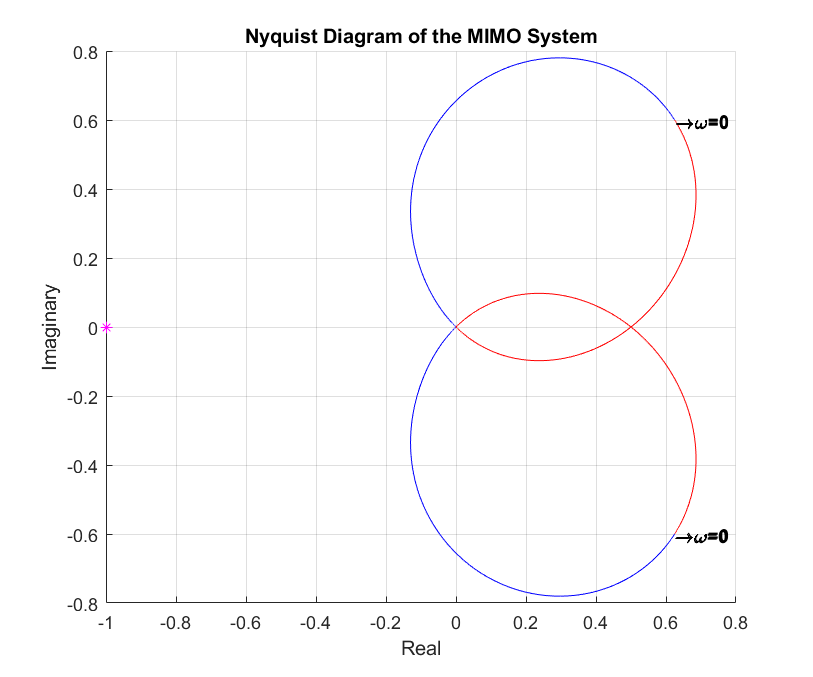
\includegraphics[width=0.55\linewidth]{char_loci_1.png}\end{center}
Neither locus encircles $-1$, and the plant has no right-half-plane poles, so by the generalised Nyquist criterion the unity-feedback loop is stable.
\end{document}
